The images were generated using the received pilots \textit{y(n)}, or in matrix form, simply  \textit{\textbf{Y}}, following the method described in \cite{Li2020}. The code to generate the images is stored in "YOLOImageGen.m" \cite{git}. After each simulated channel the following transform would be used. 

\[
    \bar{\textbf{Y}} = \textbf{U}_{\theta}^{T}  \textbf{Y} \textbf{U}_{\tau}
\]

\noindent 
Where \(\textbf{U}_{\theta}\) and \(\textbf{U}_{\tau}\) are DFT matrices with the dimensions \([\alpha \textbf{M} \text{ x } \textbf{M}]\) and \([\beta \textbf{N} \text{ x } \textbf{N}]\) respectively; where \(\alpha\) and \(\beta\) are oversampling factors. The resulting \(\bar{\textbf{Y}}\) is a delay-angle space representation of the received pilots. The oversampling factors can be used to scale up the resolution of the images, \(\bar{\textbf{Y}}\) has the dimensions \([\alpha \textbf{M} \text{ x } \beta \textbf{N}]\). Before it is displayed the \(\bar{\textbf{Y}}\) matrix is normalized as follows. 

\[
    \Tilde{\textbf{Y}} = \dfrac{\delta}{max(|\bar{\textbf{Y}}|)} |\bar{\textbf{Y}}|
\] 

\noindent 
The resulting matrix \(\Tilde{\textbf{Y}}\) has the magnitude of \(\bar{\textbf{Y}}\) scaled between 0 and \(\delta\). The new maximum value \(\delta\) scales the brightness of the points in the resulting image. With more time it would be interesting to explore how different normalization techniques would effect the generated images with different SNR ratios. The images are generated by simply displaying the  \(\Tilde{\textbf{Y}}\) matrix. The resulting images will be gray scale and show sparsity due to the number of antennas vastly out numbering the paths. Figure \ref{fig:labeledCh} shows one of the generated images with the axis labeled.
\begin{figure}[H]
\centering
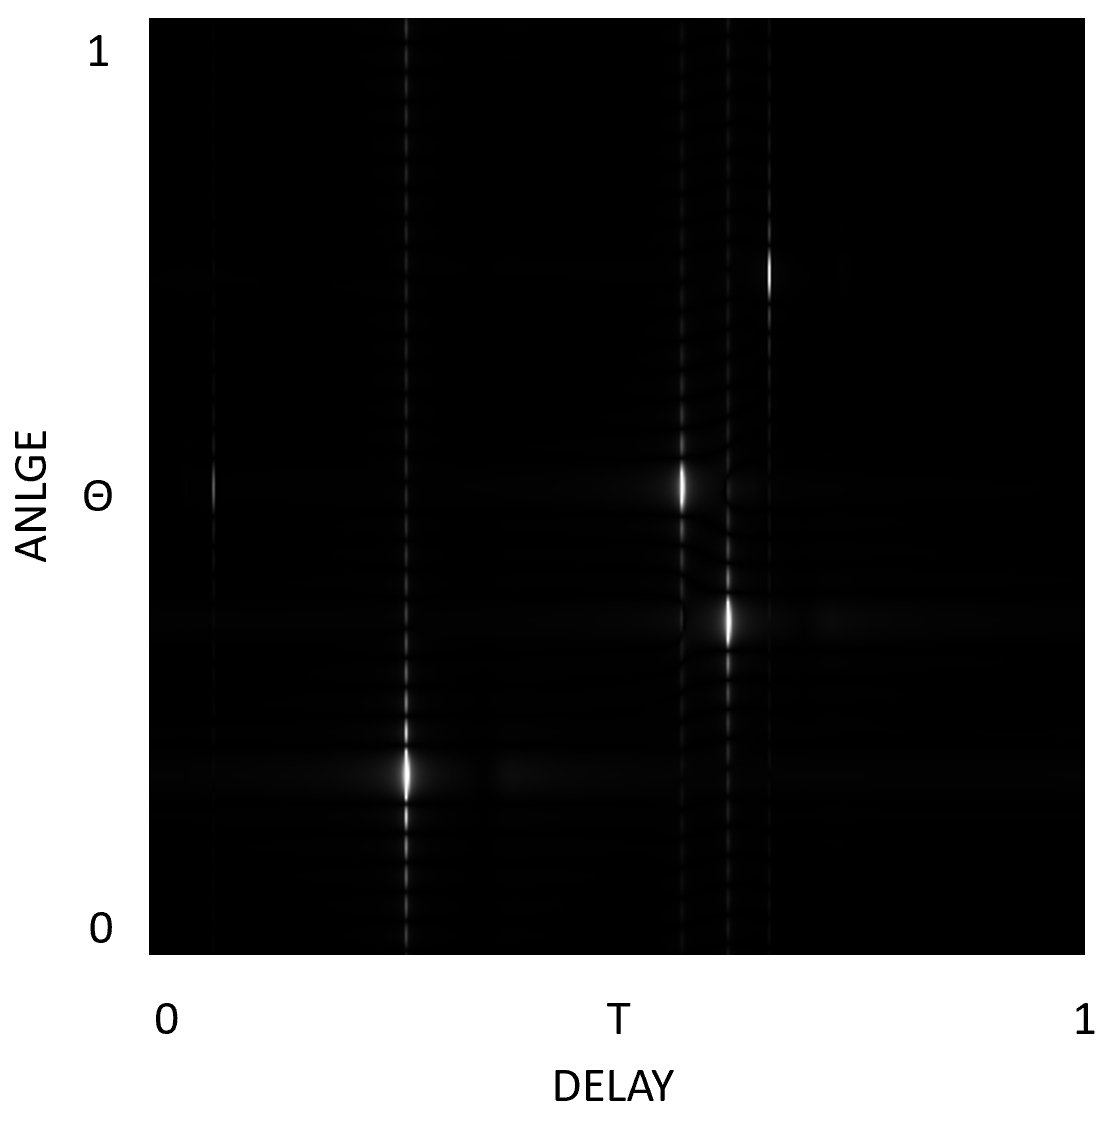
\includegraphics[width=0.5\textwidth]{figures/SYSC5804_Labeled_ChImage.png}
\caption{Labeled Channel Image}
\label{fig:labeledCh}
\end{figure}
\noindent
Each of the bright spots in the image represents a path. The coordinates of a spot are related to the antenna steering vector \(\Theta\) for the given path and the delay related phase vector \(T\). The relationship between the image and the values is shown below.

\[
    \Theta_{l} = \dfrac{y_{l}}{max(y)} - 1 
        \quad\text{and}\quad 
    T_{l} = \dfrac{y_{l}}{max(x)}
\]

\noindent 
Where \(\Theta_{l}\) and \(T_{l}\) are the value for the \(l^{th}\) path. The (\(x_{l}\), \(y_{l}\)) are the coordinates for the center point of the spot generated by the \(l^{th}\) path and (\(max(x)\), \(max(y)\)) are the width and height of the image respectively. The steering vector is subtracted by one since the image indexing starts in the top left corner. These values can be used to calculate the received angles \(\theta_{l}\) and paths delay \(\tau_{l}\) using the following equations.

\[
    \Theta_{l} =  \dfrac{d}{\lambda}\mathrm{sin}(\theta_{l})\
        \quad\text{and}\quad 
    T_{l} = \Delta f \tau_{l}
\]

\noindent
Where \(d\) is the distance between the received antennas, \(\lambda\) is the carrier wavelength, and \(\Delta f\) is the sub-carrier spacing. The \(\theta_{l}\) and $\tau_{l}$ values can be used to reconstruct the channel following the equations in Section \ref{sssec:chrec}, as is done in \cite{Han2019} and \cite{Li2020}. Unfortunately, using these equations in practice would not yield the correct path gains and delays. No matter how it was done, we could not generate the path values from the point in the image. This was disappointing, since it prevented us from closing the loop and going from received pilots all the way to a reconstructed channel.  

Varying channel conditions result in different images. Namely, changing the angle and delay of the paths changes the location of the spots in the image. Additionally, the gain of the paths is related to the brightness of the points. The SNR will also affect the image, with the noise appearing as static, the effects of varying degrees of SNR can be seen in  figure \ref{fig:snrImage}. As the SNR decreases the points become harder to recognize from the static in the background. The goal for using advanced image detection methods such as YOLO would be able to identify points in images with a lot of noise, such as figure \ref{fig:snrImage} (c). Since the image used is the normalized \(\Tilde{\textbf{Y}}\), assuming a good SNR, the dominant path is always the brightest point in the image. Other strong paths may appear dull in comparison, even if they are viable paths to transmit a signal. This can be seen in figure \ref{fig:snrImage} (a), where the LOS path is bright in the top center of the image, and another viable path is quite dim in the lower-middle right of the image. In future work we will investigate other normalization techniques to ensure the dominant path does not hide other potential paths in the image. 

\begin{figure}[H]
    \subfigure[]{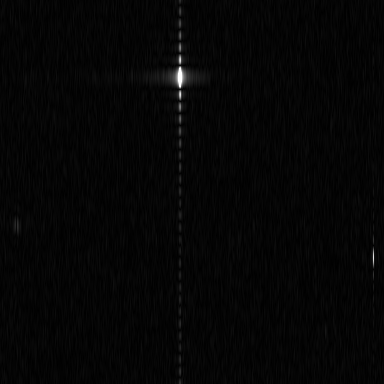
\includegraphics[width=0.245\textwidth]{SYSC5804_noNoise.png}} 
    \subfigure[]{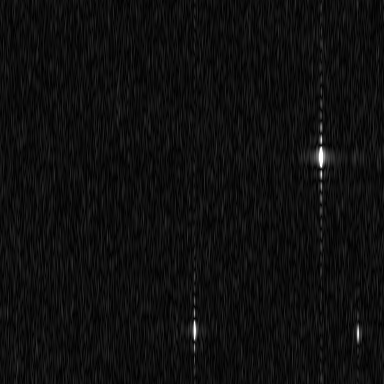
\includegraphics[width=0.245\textwidth]{SYSC5804_someNoise.png}} 
    \subfigure[]{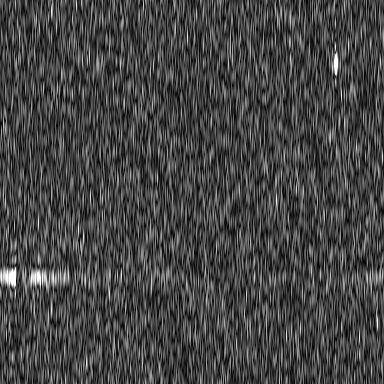
\includegraphics[width=0.245\textwidth]{SYSC5804_moreNoise.png}}
    \subfigure[]{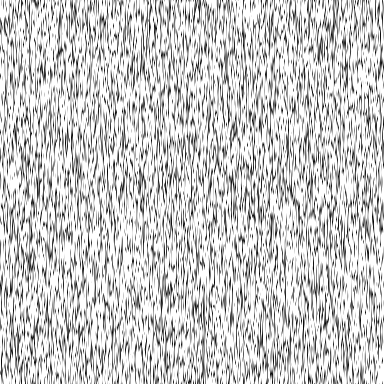
\includegraphics[width=0.245\textwidth]{SYSC5804_allNoise.png}}
    \caption{Genarated Channel Images with (a) No Noise (b) High SNR (c) Low SNR (d) Very Low SNR}
    \label{fig:snrImage}
\end{figure}

